\chapter{The Frontier Triad: Distance, Decay and Condensation}\label{ch:triad}

The compactifications of \cref{ch:k3t2,ch:tadpole,ch:stabilization} were described as
\emph{static} objects: a K3 surface, a two-torus, a set of flux integers, a minimum of a
potential. But a vacuum is only interesting if one knows what happens when it is disturbed.
Three disturbances matter most. First, one may \emph{move}: the moduli are massless fields, and
a large excursion in moduli space changes the spectrum so drastically that the effective field
theory stops making sense---this is the distance conjecture of \cref{ch:swampland}, now viewed
as a dynamical question. Second, the vacuum may \emph{decay}: a flux vacuum is only a local
minimum, and quantum mechanics lets it tunnel to a neighbouring one by nucleating a bubble;
whether this happens on cosmological time scales is governed by the sign and size of a single
number, the Euclidean bounce action. Third, the vacuum may contain an object that is simply
\emph{unstable}: a tachyon, a field sitting on top of its potential, which rolls down and
condenses. This programme packages the three questions together under the name \emph{frontier
triad}\index{frontier triad} and encodes what it assumes about each of them as a \emph{contract}:
a Lean structure or theorem that lists hypotheses explicitly and derives a conjunction of
consequences. The chapter has two aims. The first is the physics: to derive, in each of the three
cases, the inequality that decides the question---an exponential mass law, a positive bounce
action, a potential that descends to zero---with the intermediate steps written out. The second
is methodological: to explain design by contract as a way of stating a physics conjecture
in a proof assistant without pretending to prove it, and to read the four Lean files of the
triad exactly as they are, including the places where a docstring promises more than the
statement delivers.

\section{Three questions about dynamics}\label{sec:triad:three}
\index{moduli space!excursion}\index{vacuum decay}\index{tachyon}

Let us fix the setting. A compactification on $\KT$ (\cref{ch:k3t2}) or on a flux background
(\cref{ch:stabilization}) gives a four-dimensional effective theory with scalar fields
$\phi^i$, a metric $g_{ij}(\phi)$ on their target space (the moduli-space metric), and a scalar
potential $V(\phi)$, which is zero on the moduli space proper and non-zero once fluxes are
switched on. Each of the three questions is decided by a sign:

\begin{center}
\begin{tabular}{@{}p{2.8cm}p{3.6cm}p{3.2cm}p{4.6cm}@{}}
\toprule
question & quantity & condition & Lean file (\lean{.lean}) \\
\midrule
Can the moduli travel far? & tower mass $M(\phi)$ along a geodesic of length $d$ &
$M(Q)\le M(P)\,\ee^{-\alpha d}$, $\alpha>0$ & \lean{SwamplandDistance} \\
Does the vacuum last? & bounce action $B$ of the tunnelling bubble &
$B>0$ (rate $\propto\ee^{-B}$) & \lean{FluxVacuumDecay} \\
Is anything sitting on a hilltop? & tachyon potential $V(T)$ & $V''(0)<0$,
$V(T_{\min})<V(0)$ & \lean{TachyonCondensation} \\
\bottomrule
\end{tabular}
\end{center}

The three are not independent. A tachyonic direction in $V$ is exactly the second clause of the
refined de~Sitter conjecture (\cref{sec:swampland:ds}); a bubble that nucleates during vacuum
decay is itself a place where a field rolls off a hilltop; and the exponential lightening of a
tower is what eventually invalidates the effective potential in which the other two questions
are posed. The word ``frontier'' in the name records that each question sits at the edge of
what the effective theory can say about itself.

\begin{physicsbox}[What is being measured in each case]
In the first question the observable is a \emph{mass}: the lightest tower of states as a
function of position in moduli space. In the second it is a \emph{rate}: the number of bubbles
nucleated per unit four-volume, $\Gamma/V$. In the third it is an \emph{energy}: the height of
the tachyon potential above its minimum, which turns out to be the tension of the decaying
brane. None of the three is visible in the static data of a compactification; all three require
a potential or a metric on field space, i.e.\ exactly the ingredients that the lattice-theoretic
chapters of this book did not need.
\end{physicsbox}

\section{Moduli excursions and the distance conjecture}\label{sec:triad:sdc}
\index{Swampland Distance Conjecture}\index{tower of states}

\Cref{ch:swampland} derived the model case: on a circle of radius $R$, with the canonically
normalized radion $\varphi$, the Kaluza--Klein tower and the winding tower have mass scales
\begin{equation}\label{eq:triad:towers}
M_{\rm KK}\propto\ee^{+\lambda\varphi},\qquad M_w\propto\ee^{-\lambda\varphi},\qquad
M_{\rm KK}M_w=\text{const},
\end{equation}
so that whichever way $\varphi$ moves, one tower becomes light exponentially in the proper
distance $|\Delta\varphi|$, with $\lambda=\sqrt{(d-1)/(d-2)}$ in the normalization of
\eqref{eq:swampland:mkk} \source{Pal \S2.2.3, ll.~2048--2110}. Palti lists the features of this
example that the general conjecture abstracts: some tower becomes light for either sign of
$\Delta\varphi$; the phenomenon is stringy, because one tower consists of winding states absent
in field theory; the product of the two scales is independent of $\varphi$; the exponent is of
order one; and as $|\Delta\varphi|\to\infty$ infinitely many states become massless, so that no
$d$-dimensional field theory describes that locus \source{Pal \S2.2.3, ll.~2110--2135}.

The conjecture itself, in its original form, has two parts \source{Pal \S2.2.3,
ll.~2165--2183}: (i) from any point $P$ of a moduli space $\mathcal M$ there is a point $Q$ at
infinite geodesic distance $d(P,Q)$; (ii) there is an infinite tower with mass scale
\begin{equation}\label{eq:triad:sdc}
M(Q)\sim M(P)\,\ee^{-\alpha\,d(P,Q)},\qquad\alpha>0 .
\end{equation}
The refined form replaces $\sim$ by a strict inequality and reinstates the Planck mass
\source{Pal \S3.6, ll.~5154--5175}:
\begin{equation}\label{eq:triad:rsdc}
M(Q)<M(P)\,\ee^{-\alpha\,d(P,Q)/M_p}\qquad\text{for }d(P,Q)\gtrsim M_p ,
\end{equation}
with the exponential behaviour setting in ``at $1$--$2\,M_p$'' and no way to delay it, and
holding also for fields with a potential, the moduli space being replaced by the field space
of the effective theory \source{Pal \S3.6, ll.~5176--5200}.

\subsection{From a mass law to a range of validity}

What makes \eqref{eq:triad:rsdc} a statement about \emph{dynamics} is the following
consequence. Suppose an effective theory with cutoff $\Lambda$ is written down at the point $P$,
where the lightest tower has scale $M(P)>\Lambda$. The theory can only be used where the tower
is still above the cutoff, $M(\phi)>\Lambda$. Combining with \eqref{eq:triad:rsdc},
\begin{equation}\label{eq:triad:range}
\Lambda<M(\phi)<M(P)\,\ee^{-\alpha d/M_p}\quad\Longrightarrow\quad
d(P,\phi)<\frac{M_p}{\alpha}\,\ln\frac{M(P)}{\Lambda}.
\end{equation}
This is the ``continuous analogue'' Palti mentions: a field theory with a cutoff below an
infinite tower holds only on a finite range of expectation values \source{Pal \S2.2.3,
ll.~2136--2140}. The range grows only logarithmically with the hierarchy $M(P)/\Lambda$, and is
inversely proportional to $\alpha$. This is why the value of $\alpha$ matters and why the
refined conjecture insists on an implicit lower bound for it \source{Pal \S3.6,
ll.~5177--5190}: an $\alpha\ll1$ would let the moduli travel many Planck units without much
change in the spectrum, and the conjecture would lose its bite.

\begin{example}[Halving distances]\label{ex:triad:halving}
The Lean file \lean{SwamplandDistance.lean} stipulates the value $\alpha=1/\sqrt2$ (as the
rational identity $2\alpha^2=1$, \cref{sec:triad:lean}). With this value, the distance over
which the tower mass halves is
\[
d_{1/2}=\frac{M_p\ln2}{\alpha}=\sqrt2\,\ln2\,M_p\approx0.98\,M_p ,
\]
and after $d=1,2,3$ Planck units the suppression factors are
$\ee^{-1/\sqrt2}\approx0.49$, $\ee^{-\sqrt2}\approx0.24$, $\ee^{-3/\sqrt2}\approx0.12$.
If the tower starts at $M(P)=M_p$ and the effective theory is to describe physics up to
$\Lambda=10^{-2}M_p$, then \eqref{eq:triad:range} allows
$d<\sqrt2\ln100\,M_p\approx6.5\,M_p$. For the circle in $d=4$ the exponent is instead
$\lambda=\sqrt{3/2}\approx1.22$ in the normalization of \eqref{eq:swampland:mkk}, or
$\lambda/\sqrt2\approx0.87$ in Palti's normalization (\cref{sec:swampland:circle}); the number
$1/\sqrt2$ is neither, and nothing in the Lean file connects it to a tower. It should be read
as a placeholder for ``some $\alpha$ of order one''.
\end{example}

\begin{physicsbox}[The dual-scale reading]
On the circle, the product $M_{\rm KK}M_w$ in \eqref{eq:triad:towers} is constant because
$M_{\rm KK}\propto1/R$ and $M_w\propto R/\ap$. The lightest of the two scales is
$\min(1/R,R/\ap)$, maximal at the self-dual radius $R=\sqrt{\ap}$, and this is the same
statement as $R+\ap/R\ge2\sqrt{\ap}$ of \cref{ch:dualscale}: the sum is smallest exactly where
the lightest tower is heaviest. The distance conjecture says that the effective theory is
healthiest in the middle of moduli space and degenerates at every end; the dual-scale
inequality says the same for the one-dimensional case in the language of $R$ rather than of
$\varphi$. Which of the two towers becomes light is decided by the sign of $\Delta\varphi$,
and T-duality is the $\Z_2$ that exchanges them \source{Pal \S2.2.3, ll.~2141--2160}.
\end{physicsbox}

\section{Flux vacuum decay and the bounce}\label{sec:triad:decay}
\index{Coleman--De Luccia instanton}\index{bounce action}\index{thin-wall approximation}

The flux superpotential of \cref{ch:stabilization} produces, for each choice of flux integers,
a local minimum of $V$. Neighbouring minima differ by one unit of some flux, and a transition
between them is mediated by the nucleation of a brane (a domain wall in four dimensions)
across which the flux jumps. Giddings, Kachru and Polchinski use the same physics in a different
role: interactions between modes localized in distinct warped throats are
``tunneling-suppressed (and therefore weak)'' \source{GKP \S5, ll.~1605--1611}. Here we need
the suppression itself. The question is: given a false vacuum with energy density $V_+$ and a
true vacuum with $V_-<V_+$, separated by a wall of tension $\sigma$, how often does a bubble of
true vacuum appear?

\subsection{The thin-wall bounce}

The semiclassical answer is standard; it is not in this book's source library and we derive it
on the page (``standard; not checked against a source in this book's library''). The rate per
unit volume is
\begin{equation}\label{eq:triad:rate}
\frac{\Gamma}{V}=A\,\ee^{-B},\qquad B=S_E[\text{bounce}]-S_E[\text{false vacuum}],
\end{equation}
where $S_E$ is the Euclidean action and the bounce is the $O(4)$-symmetric solution of the
Euclidean equations of motion that interpolates from the true vacuum at the centre to the
false vacuum at infinity. When the energy difference $\epsilon=V_+-V_-$ is small compared with
the barrier, the bubble is large and its wall is thin, and the action is a function of a single
number, the bubble radius $R$. Two contributions compete: the wall costs energy proportional to
its area, and the interior gains energy proportional to its volume. In four Euclidean
dimensions a ball of radius $R$ has volume $\tfrac{\pi^2}{2}R^4$ and its boundary three-sphere
has area $2\pi^2R^3$, so
\begin{equation}\label{eq:triad:BR}
B(R)=2\pi^2R^3\sigma-\frac{\pi^2}{2}R^4\epsilon .
\end{equation}
The bounce is the stationary point of $B(R)$:
\begin{equation}\label{eq:triad:Rstar}
\frac{\dd B}{\dd R}=6\pi^2R^2\sigma-2\pi^2R^3\epsilon=0\quad\Longrightarrow\quad
R_*=\frac{3\sigma}{\epsilon},
\end{equation}
and substituting back,
\begin{equation}\label{eq:triad:bounce}
B_*=2\pi^2\frac{27\sigma^4}{\epsilon^3}-\frac{\pi^2}{2}\,\frac{81\sigma^4}{\epsilon^3}
=\frac{\pi^2\sigma^4}{\epsilon^3}\Big(54-\frac{81}{2}\Big)=\frac{27\pi^2\sigma^4}{2\epsilon^3}.
\end{equation}
(Symbolic check: sympy reproduces $R_*$ and $B_*$ from \eqref{eq:triad:BR}.) Two features
deserve comment. First, $B''(R_*)=-18\pi^2\sigma^2/\epsilon<0$: the stationary point is a
\emph{maximum} of $B(R)$, as it must be---a bubble smaller than $R_*$ shrinks, a larger one
grows, and the bounce is the critical bubble that does neither. It is a saddle of the full
action, with exactly one negative mode, and that negative mode is what makes the false vacuum's
energy acquire an imaginary part, i.e.\ a decay rate. Second, $B_*>0$ whenever $\sigma>0$ and
$\epsilon>0$: the rate is exponentially suppressed, and the suppression becomes infinite as the
two vacua become degenerate, $\epsilon\to0$. The vacuum is then stable, not because tunnelling
is forbidden, but because the critical bubble becomes infinitely large.

\begin{figure}[ht]
\centering
\begin{tikzpicture}[scale=1]
\draw[->] (0,0) -- (6.4,0) node[right] {$R$};
\draw[->] (0,-0.8) -- (0,3.2) node[above] {$B(R)$};
% B(R) with sigma/epsilon = 1: B ∝ R^3 (4 - R), maximum 27 at R = 3; scaled to height 2.4
\draw[thick,blue!60!black,domain=0:4.15,samples=80] plot (\x,{(\x)^3*(4-\x)*2.4/27});
\draw[dashed] (3,0) -- (3,2.4);
\draw[dashed] (0,2.4) -- (3,2.4);
\node[below] at (3,0) {$R_*=3\sigma/\epsilon$};
\node[left] at (0,2.4) {$B_*$};
\node[anchor=west] at (0.3,2.9) {\small wall term $+2\pi^2\sigma R^3$ dominates};
\node[anchor=west] at (4.2,1.2) {\small volume term $-\tfrac{\pi^2}{2}\epsilon R^4$ dominates};
\end{tikzpicture}
\caption{The thin-wall action \eqref{eq:triad:BR} as a function of the bubble radius. The
bounce sits at the maximum $R_*=3\sigma/\epsilon$; bubbles to the left collapse, bubbles to the
right expand and convert the false vacuum.}
\label{fig:triad:bounce}
\end{figure}

\begin{example}[Numbers for a flux step]\label{ex:triad:bouncenumbers}
Measure $\sigma$ in units of $M^3$ and $\epsilon$ in units of $M^4$ for some scale $M$. For
$\sigma=1$, $\epsilon=0.1$ the critical radius is $R_*=30/M$ and $B_*=27\pi^2\cdot10^3/2
\approx1.3\times10^5$, so $\Gamma/V\propto\ee^{-1.3\times10^5}$---for all purposes the vacuum
is eternal. For $\sigma=1$, $\epsilon=0.5$ one finds $R_*=6/M$ and $B_*\approx1.07\times10^3$;
for $\sigma=2$, $\epsilon=1$, again $R_*=6/M$ but $B_*\approx2.1\times10^3$, twice as large
because $B_*$ scales as $\sigma^4/\epsilon^3$ and both have doubled. The lesson is the extreme
sensitivity to the wall tension: at fixed $\epsilon$, doubling $\sigma$ multiplies the exponent
by $16$.
\end{example}

\subsection{Gravity and the arrow of the decay}

With gravity, the bubble geometry itself changes, and the bounce action of
\eqref{eq:triad:bounce} receives corrections controlled by $R_*/M_p$ times powers of
$\sqrt{V/M_p^2}$; the classic result is that decay of a Minkowski or de~Sitter vacuum to a
vacuum of lower energy remains possible, while decay out of a supersymmetric Minkowski vacuum is
forbidden. Neither statement is in this book's library and we do not use them. What we do use
is the direction of the process: a decay $V_+\to V_-$ lowers the energy density, and in the flux
landscape it lowers the flux integer $N+1\to N$ by one unit. The Lean file
\lean{FluxVacuumDecay.lean} records both directions as strict inequalities on integers, with a
docstring that invokes a holographic $c$-theorem to interpret the second; \cref{sec:triad:lean}
explains why that interpretation is not part of what is proved.

\begin{pitfallbox}[A positive bounce action is not a stable vacuum]
$B>0$ means only that the rate is \emph{suppressed}, $\Gamma/V\propto\ee^{-B}$, not that it is
zero. Whether a vacuum is stable on the age of the universe depends on the value of $B$
compared with $\ln(\text{Hubble volume}\times\text{age})$, i.e.\ on a number of order a few
hundred, and on the prefactor $A$, which has dimension mass$^4$ and is set by the fluctuation
determinant around the bounce. A Lean theorem that proves $B>0$ has proved the least
interesting of the three facts (sign, magnitude, prefactor).
\end{pitfallbox}

\section{Tachyons and condensation}\label{sec:triad:tachyon}
\index{tachyon!as hilltop field}\index{tachyon condensation}\index{Sen conjecture}

\subsection{What a negative mass squared means}

The bosonic closed string's ground state has \source{Tong \S2.3.1, ll.~2535--2545}
\begin{equation}\label{eq:triad:closedtachyon}
M^2=-\frac{1}{\ap}\,\frac{D-2}{6}\;\;\xrightarrow{\;D=26\;}\;\;M^2=-\frac4{\ap} ,
\end{equation}
and the bosonic open string on a D$p$-brane has $M^2=-1/\ap$, ``half that of the closed string
tachyon'' in the sense of $|M^2|$ \source{Tong \S3.1.1, ll.~3312--3320}. Tong's interpretation
is the one to keep \source{Tong \S2.3.1, ll.~2546--2566}: the mass squared of a particle is
the quadratic coefficient of the potential of the field $T(X)$ that creates it,
\begin{equation}\label{eq:triad:msq}
M^2=\frac{\partial^2V(T)}{\partial T^2}\Big|_{T=0},
\end{equation}
so a negative $M^2$ says that the theory has been expanded about a \emph{maximum} of $V$. The
Higgs field at $H=0$ is a tachyon in exactly this sense. The question is then whether $V$ has a
good minimum elsewhere. For the closed-string tachyon Tong reports that the answer is unknown:
the cubic term produces a minimum, the quartic destabilizes it again, and $T$ mixes with the
other scalars \source{Tong \S2.3.1, ll.~2566--2590}. For the open-string tachyon the picture is
different and, by now, well understood \source{Tong \S3.1.1, ll.~3319--3340}: the brane is
unstable, it decays ``by dissolving into closed string modes'', the end point is ``a state with
no D-brane'', and
\begin{equation}\label{eq:triad:tension}
V(0)-V(T_{\min})=\tau_p ,
\end{equation}
the tension of the D-brane. This is Sen's conjecture on the open-string tachyon potential.

\subsection{A model potential and two consistency checks}

A frequently used closed form for the potential of the tachyon on an unstable D-brane of the
superstring is
\begin{equation}\label{eq:triad:senV}
V(T)=\frac{\tau_p}{\cosh(T/\sqrt2)}\qquad(\ap=1),
\end{equation}
which the Lean file \lean{UseCase3\_FrontierTriad.lean} quotes in its docstring; it is
``standard; not checked against a source in this book's library''. Two checks show that it is at
least the right shape. First, $V(0)=\tau_p$ and $V(T)\to0$ as $|T|\to\infty$, so
$V(0)-V(\infty)=\tau_p$, which is \eqref{eq:triad:tension} with the minimum at infinity.
Second, expanding $1/\cosh x=1-x^2/2+\dots$ gives $V(T)=\tau_p(1-T^2/4+\dots)$, so by
\eqref{eq:triad:msq}
\begin{equation}\label{eq:triad:sencheck}
M^2=V''(0)/\tau_p=-\tfrac12\quad\text{in units }\ap=1,\qquad\text{i.e. } M^2=-\frac1{2\ap},
\end{equation}
provided the kinetic term is normalized as $\tfrac12\tau_p(\partial T)^2$ near $T=0$. This is
the mass of the tachyon on a non-BPS brane or a brane--antibrane pair of the superstring (as
stated, without derivation, in the docstring of \lean{TachyonCondensation.lean}). It differs
from the bosonic open-string value $-1/\ap$ quoted above by a factor two, as it should: these
are different theories. (Symbolic check: sympy gives $V(0)=1$, $V(\infty)=0$, $V''(0)=-1/2$ for
$\tau_p=1$.)

\begin{figure}[ht]
\centering
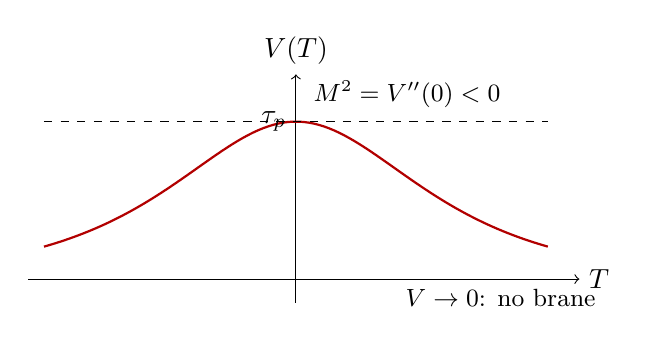
\begin{tikzpicture}[scale=1]
\draw[->] (-3.4,0) -- (3.6,0) node[right] {$T$};
\draw[->] (0,-0.3) -- (0,2.6) node[above] {$V(T)$};
\draw[thick,red!70!black,domain=-3.2:3.2,samples=100] plot (\x,{2/cosh(\x/1.4142)});
\draw[dashed] (-3.2,2) -- (3.2,2);
\node[left] at (0,2) {$\tau_p$};
\node[above right] at (0.1,2.05) {\small $M^2=V''(0)<0$};
\node[below] at (2.6,0) {\small $V\to0$: no brane};
\end{tikzpicture}
\caption{The model potential \eqref{eq:triad:senV}. The unstable brane sits at the top,
$V(0)=\tau_p$; the tachyon rolls to $|T|\to\infty$ where the energy stored in the brane has
been released. The height of the hill is the brane tension, \eqref{eq:triad:tension}.}
\label{fig:triad:senV}
\end{figure}

\subsection{Brane--antibrane pairs and what survives condensation}

For a coincident D$p$--$\overline{\mathrm{D}p}$ pair the tachyon is a complex field, and if it
condenses with a non-trivial winding at infinity the end point is not empty space but a
lower-dimensional brane. The bookkeeping that survives is a \emph{charge}: the pair carries the
formal difference $[E]-[F]$ of the bundles on the brane and antibrane, and the defect left
behind carries the same class. This is Witten's K-theoretic classification of D-brane charge,
cited in the docstring of \lean{TachyonCondensation.lean} but not in this book's library; we
use only the arithmetic consequence that the rank and the Chern numbers of $[E]-[F]$ are
differences of those of $E$ and $F$, which is a definition. The physical statement---that the
soliton at the end of condensation carries exactly this class---is Tier~L on the authority of
that literature, and the Lean theorem named after it is a tautology (\cref{sec:triad:lean}).

\subsection{The tachyon in the refined de Sitter conjecture}

The refined de~Sitter conjecture of \cref{ch:swampland} says that a potential in the landscape
satisfies either $|\nabla V|\ge cV/M_p$ or
\begin{equation}\label{eq:triad:rds}
\min\big(\nabla_i\nabla_jV\big)\le-\frac{c'}{M_p^2}\,V ,
\end{equation}
the minimum eigenvalue of the Hessian in an orthonormal frame \source{Pal \S7,
ll.~10558--10575}. The second clause is precisely a tachyon condition: a direction in field
space with negative mass squared, of magnitude at least $c'V/M_p^2$. It was introduced because
the first clause alone is violated at the top of the Higgs potential, where
$|\nabla V|/V\sim10^{-55}/M_p$ while the Hessian is enormously negative,
$\sim-10^{35}V/M_p^2$ \source{Pal \S7, ll.~10590--10603}; the refined conjecture ``is
certainly satisfied'' there. So the third member of the triad, condensation, enters the
swampland programme as the escape clause of the de~Sitter conjecture: hilltops are allowed,
provided they are steep enough that the field does not linger.

\begin{pitfallbox}[Tachyons do not travel faster than light]
The special-relativistic picture of a tachyon as a particle with $v>c$ is ``not the right
interpretation'' \source{Tong \S2.3.1, ll.~2547--2556}. In field theory a negative $M^2$
is an instability of the vacuum, not a superluminal signal: perturbations grow exponentially
in time rather than oscillating, and the theory must be re-expanded about the true minimum.
The string-gas literature makes the same point in reverse: the ``tachyonic zero point energy''
of the bosonic string is removed by hand from the mass formula before any thermodynamics is
done, because it would be absent in the heterotic string anyway \source{BW \S III, ll.~886--890}.
\end{pitfallbox}

\section{Design by contract for physics conjectures}\label{sec:triad:contract}
\index{design by contract}\index{contract (Lean)}\index{conjecture!as hypothesis}

None of the three inequalities above is a theorem of mathematics. The distance conjecture is a
conjecture; the positivity of the bounce action depends on a semiclassical approximation and
on the signs of $\sigma$ and $\epsilon$; Sen's conjecture is established by string field theory
calculations, not by a proof. How, then, should a proof assistant handle them? \Cref{ch:swampland}
gave the general answer: encode the conjecture's \emph{shape} as a structure or a hypothesis and
prove what follows. This programme's name for the pattern is a \emph{contract}, borrowed from
software engineering, where a routine is specified by a precondition (what the caller must
guarantee) and a postcondition (what the routine then guarantees). Translated to Lean:

\begin{definition}[Contract]\label{def:triad:contract}
A \emph{contract} for a physical statement is a Lean declaration of the form
\[
\texttt{theorem}\ \textit{name}\ (x_1:\alpha_1)\cdots(x_k:\alpha_k)\ (h_1:P_1)\cdots(h_m:P_m)\;:\;
Q_1\wedge Q_2\wedge\cdots\wedge Q_r ,
\]
whose parameters $x_i$ are the data of the problem, whose hypotheses $h_j$ are the physical
assumptions made explicit, and whose conclusion is the conjunction of the consequences drawn.
A \emph{master contract} is one whose conjuncts are themselves the conclusions of separately
proved theorems, so that its proof is an assembly, \lean{⟨thm₁, thm₂, thm₃⟩}.
\end{definition}

The value of the pattern lies in what it forces one to write down. Every assumption is a named
hypothesis; every consequence is a proposition that must type-check against the definitions;
and the kernel refuses any step that uses an assumption not in the list. The pattern does
\emph{not} guarantee that the assumptions are the physically relevant ones, nor that the
definitions capture the physics. Three failure modes recur in the libraries of this book and
the reader should learn to recognize them on sight:

\begin{enumerate}[leftmargin=2em,itemsep=2pt]
\item \textbf{Vacuous conclusion.} The conclusion is \lean{True} or an equation between literals
provable by \lean{rfl}. The hypotheses may be physically meaningful, but the theorem uses none of
them. \Cref{ch:swampland}'s \lean{de\_sitter\_conjecture} is the extreme case.
\item \textbf{Stipulated dynamics.} A quantity that physics would compute---a bounce action, a
tower mass---is \emph{defined} to have the property that the theorem then ``proves''. The proof
is correct, the content is the definition, and the definition is a modelling choice.
\item \textbf{Unused hypotheses.} A hypothesis is listed in the signature but the proof never
refers to it. Lean's linter flags this; the physical reading is that the conclusion is weaker
than the name suggests.
\end{enumerate}

\begin{physicsbox}[How to read a contract]
Read the conclusion first, then the definitions it unfolds to, then the hypotheses, then the
name. Ask: if I replace each defined constant by a variable, does the theorem still go through?
If yes, the theorem is about the \emph{form} of the statement (good: that is what a contract is
for). If no, the theorem is about specific numbers, and it is a computation, not a law. Both are
legitimate; only the reading changes.
\end{physicsbox}

\begin{example}[The master contract of the triad]\label{ex:triad:master}
In the file \lean{UseCase3\_FrontierTriad.lean} the theorem\\
\lean{frontier\_triad\_master\_contract}
has the form of \cref{def:triad:contract} with data $(m_0,t_b)\in\N^2$, one hypothesis
$t_b\ge1$, and three conjuncts: the RR tadpole of the $\KT/\Z_2$ orientifold vanishes; the
tower mass after one ``halving'' is at most $m_0$; the numerator of the thin-wall bounce action
is positive. Its proof is exactly the assembly $\langle\text{tadpole},\text{sdc},
\text{bounce}\rangle$. Applying the reading rule: the first conjunct is an equation between
literals ($64-64=0$, failure mode 1 in a mild form---it is a genuine tadpole computation but
does not depend on the parameters); the second is $m_0/2\le m_0$ in natural-number division,
a true statement about the form $m\mapsto m/k$ that survives replacing $2$ by any $k\ge1$; the
third is $27t_b^4>0$, which needs the hypothesis $t_b\ge1$ and uses it. The contract is
honest about its inputs and modest in its outputs, and that is the best one can say of any
formalization of a conjecture.
\end{example}

\begin{figure}[ht]
\centering
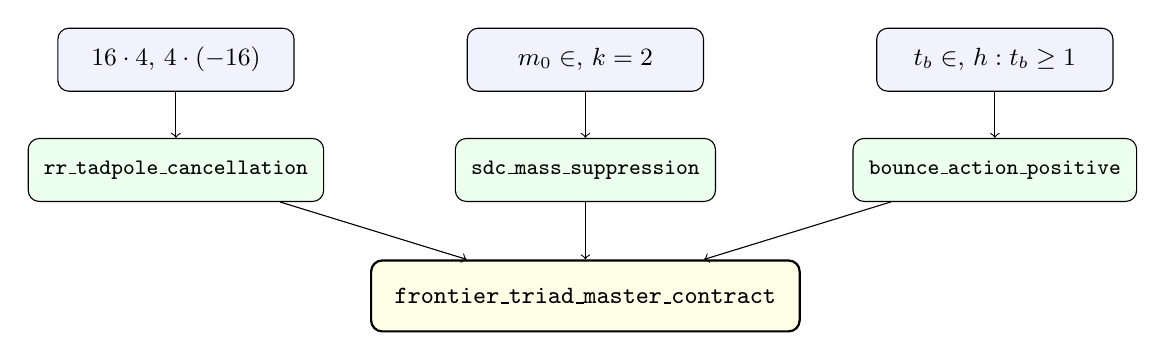
\begin{tikzpicture}[
  hyp/.style={draw,rounded corners,fill=blue!5,minimum width=3.0cm,minimum height=8mm,font=\small},
  thm/.style={draw,rounded corners,fill=green!7,minimum height=8mm,font=\footnotesize\ttfamily,inner xsep=2mm},
  master/.style={draw,thick,rounded corners,fill=yellow!10,minimum height=9mm,font=\small\ttfamily\bfseries,inner xsep=3mm}]
\node[hyp] (d) at (0,2.4) {$16\cdot4$, $4\cdot(-16)$};
\node[hyp] (m) at (5.2,2.4) {$m_0\in\N$, $k=2$};
\node[hyp] (t) at (10.4,2.4) {$t_b\in\N$, $h:t_b\ge1$};
\node[thm] (T1) at (0,1) {rr\_tadpole\_cancellation};
\node[thm] (T2) at (5.2,1) {sdc\_mass\_suppression};
\node[thm] (T3) at (10.4,1) {bounce\_action\_positive};
\node[master] (M) at (5.2,-0.6) {frontier\_triad\_master\_contract};
\draw[->] (d) -- (T1); \draw[->] (m) -- (T2); \draw[->] (t) -- (T3);
\draw[->] (T1) -- (M); \draw[->] (T2) -- (M); \draw[->] (T3) -- (M);
\end{tikzpicture}
\caption{Anatomy of the master contract: data and hypotheses (top), three component theorems
(middle), and their conjunction (bottom). Only the right-hand column carries a hypothesis
that the proof actually uses.}
\label{fig:triad:contract}
\end{figure}

\section{What the machine has checked}\label{sec:triad:lean}
\index{Lean!frontier triad}\index{arithmetic shadow}

Four files carry the triad: three in \lean{DualScaleM24Formalization/FrontierTriad/} and the
use case \lean{DualScaleValidation/UseCase3\_FrontierTriad.lean}, which imports the first of
them together with the Kummer tadpole file of \cref{ch:tadpole}. All compile with no
\lean{sorry} and depend only on the three standard axioms. Every statement below is quoted from
the file; the proofs are omitted. We take the files in the order of the chapter.

\subsection{Distance: \lean{SwamplandDistance.lean}}

The moduli-dimension arithmetic ($58$, $80$) and the Boolean predicate
\lean{isSwamplandSafe} of this file were read in \cref{ch:swampland}, and \cref{ch:k3t2}
explained why $80$ is the dimension of the K3 sigma-model moduli space rather than of $\KT$.
What remains for us is the decay coefficient:
\begin{leancode}
/-- SDC decay rate coefficient α = 1/√2 numerator of α²: 1. -/
def sdc_decay_alpha_squared_num : Nat := 1
/-- SDC decay rate coefficient α = 1/√2 denominator of α²: 2. -/
def sdc_decay_alpha_squared_den : Nat := 2

theorem sdc_decay_coefficient_identity :
    2 * sdc_decay_alpha_squared_num = sdc_decay_alpha_squared_den := by rfl

def fricke_N : Int := 1
def fricke_square : Int := fricke_N * fricke_N
theorem fricke_involution_property : fricke_square = 1 := by rfl
def fricke_discriminant : Int := 0 - 4 * 1 * 1
theorem fricke_discriminant_is_minus_four : fricke_discriminant = -4 := by rfl
\end{leancode}
\begin{leanbox}[Plain-language reading]
\lean{sdc\_decay\_coefficient\_identity} says $2\cdot1=2$. The docstring reads this as
$2\alpha^2=1$ with $\alpha=1/\sqrt2$, but no real number, no square root and no tower appear
in the statement; the two naturals are \emph{named} as numerator and denominator of
$\alpha^2$ and nothing enforces the name. \lean{fricke\_involution\_property} says $1\cdot1=1$
and \lean{fricke\_discriminant\_is\_minus\_four} says $0-4=-4$; the docstring's ``Fricke
involution $W_1^2=\mathrm{Id}$'' and ``discriminant of $x^2+1$ at the fixed point $\tau=\ii$''
are the intended meanings, and the second is indeed the discriminant $b^2-4ac$ of
$x^2+0x+1$. Proof idea in every case: \lean{rfl}, definitional unfolding of literals. This is
failure mode 2 of \cref{sec:triad:contract} in its purest form; what would be needed to make
$\alpha$ a theorem is described in \cref{ch:swampland}.
\end{leanbox}

\subsection{Decay: \lean{FluxVacuumDecay.lean}}

\begin{leancode}
structure FluxVacuum where
  fluxNumber : Nat
  energyScale : Nat
  centralCharge : Nat

def standardFluxVacuum (n : Nat) : FluxVacuum := {
  fluxNumber := n
  energyScale := 100 * (n + 1)
  centralCharge := 100 * (n + 1)
}

structure CDLInstanton where
  falseVacuum : FluxVacuum
  trueVacuum : FluxVacuum
  bounceAction : Nat

def unitFluxDecay (n : Nat) : CDLInstanton := {
  falseVacuum := standardFluxVacuum (n + 1)
  trueVacuum := standardFluxVacuum n
  bounceAction := 42 * (n + 1)
}

theorem cdl_action_strictly_positive (n : Nat) :
    (unitFluxDecay n).bounceAction > 0 := by ...
theorem true_vacuum_energy_is_lower (n : Nat) :
    (unitFluxDecay n).falseVacuum.energyScale
      > (unitFluxDecay n).trueVacuum.energyScale := by ...
theorem holographic_c_theorem_decay (n : Nat) :
    (unitFluxDecay n).trueVacuum.centralCharge
      < (unitFluxDecay n).falseVacuum.centralCharge := by ...
\end{leancode}
\begin{leanbox}[Plain-language reading]
A \lean{FluxVacuum} is a triple of natural numbers; \lean{standardFluxVacuum n} is
$(n,\,100(n+1),\,100(n+1))$; a \lean{CDLInstanton} is a pair of such triples with a third
natural number called the bounce action; \lean{unitFluxDecay n} is the instanton from
$(n+1,100(n+2),100(n+2))$ to $(n,100(n+1),100(n+1))$ with bounce action $42(n+1)$. The three
theorems say, for every $n\in\N$: $42(n+1)>0$; $100(n+2)>100(n+1)$; $100(n+1)<100(n+2)$. Proof
idea: unfold the definitions (\lean{dsimp}) and let \lean{omega}, the decision procedure for
linear arithmetic over $\N$ and $\Z$, close the goal. \emph{What is not here}: no potential, no
Euclidean action, no bubble, no $\sigma$ or $\epsilon$, and therefore no
\eqref{eq:triad:bounce}; the bounce action is stipulated to be $42(n+1)$ (failure mode~2). The
second and third theorems are the same inequality about the same function $100(n+1)$ under two
names; the docstring's ``holographic $c$-theorem'' and ``arrow of time'' are interpretations
of the label \lean{centralCharge}, which the kernel never sees. A faithful formalization of
\cref{sec:triad:decay} would take $\sigma,\epsilon>0$ real, define $B(R)$ by
\eqref{eq:triad:BR}, and prove that $R_*=3\sigma/\epsilon$ is its unique positive critical
point with $B(R_*)=27\pi^2\sigma^4/(2\epsilon^3)>0$; \cref{exe:triad:leanbounce} asks for the
first step.
\end{leanbox}

\subsection{Condensation: \lean{TachyonCondensation.lean}}

\begin{leancode}
structure KClass where
  rank : Int
  firstChern : Int
  secondChern : Int

def kSub (a b : KClass) : KClass := {
  rank := a.rank - b.rank
  firstChern := a.firstChern - b.firstChern
  secondChern := a.secondChern - b.secondChern
}

structure BraneAntiBraneSystem where
  braneE : KClass
  antiBraneF : KClass
  tachyonVEV : Nat
  is_annihilated : Bool

def systemKTheoryClass (sys : BraneAntiBraneSystem) : KClass :=
  kSub sys.braneE sys.antiBraneF

structure SenSolitonDefect where
  dimension : Nat
  worldvolumeDefect : KClass
  solitonCenter : Nat

def condenseTachyon (sys : BraneAntiBraneSystem) (dim : Nat) :
    SenSolitonDefect := {
  dimension := dim
  worldvolumeDefect := systemKTheoryClass sys
  solitonCenter := 0
}

theorem sen_conjecture_k_theory_conservation
    (sys : BraneAntiBraneSystem) (dim : Nat) :
    (condenseTachyon sys dim).worldvolumeDefect
      = systemKTheoryClass sys := by rfl

def rrCharge (k : KClass) : Int :=
  k.rank + k.firstChern + k.secondChern

theorem tachyon_condensation_preserves_rr_charge
    (sys : BraneAntiBraneSystem) (dim : Nat) :
    rrCharge (condenseTachyon sys dim).worldvolumeDefect
      = rrCharge (systemKTheoryClass sys) := by rfl
\end{leancode}
\begin{leanbox}[Plain-language reading]
A \lean{KClass} is a triple of integers $(r,c_1,c_2)$ and \lean{kSub} subtracts componentwise;
this is the correct arithmetic of rank and Chern numbers in the Grothendieck group, where
$[E]-[F]$ has rank $\rk E-\rk F$ and Chern character $\mathrm{ch}(E)-\mathrm{ch}(F)$ (Tier~L;
the component formula is a definition once one accepts that $\mathrm{ch}$ is additive). The
function \lean{condenseTachyon} \emph{copies} $[E]-[F]$ into the field
\lean{worldvolumeDefect} of the output. The theorem
\lean{sen\_conjecture\_k\_theory\_conservation} then says that the copy equals the original,
and \lean{tachyon\_condensation\_preserves\_rr\_charge} says that a function applied to the
copy equals the same function applied to the original; both are \lean{rfl}. These are
tautologies by construction: the physical claim that condensation \emph{produces} a defect in
class $[E]-[F]$ has been put into the definition of \lean{condenseTachyon}, so the theorem
cannot fail. Note also that \lean{tachyonVEV} and \lean{is\_annihilated} are never read, that
\lean{rrCharge} adds a rank to two Chern numbers without the powers of $2\pi$ or the
$\sqrt{\hat A}$ factor that a Chern-character integral would carry, and that no potential
$V(T)$ appears anywhere, so \eqref{eq:triad:tension} and \eqref{eq:triad:sencheck} are not
represented. The docstring's mass $m^2=-1/(2\ap)$ is correct for the superstring
brane--antibrane tachyon (\cref{sec:triad:tachyon}) but is not a statement of the file.
\end{leanbox}

\subsection{Gates and a graph invariant: \lean{TriadContract.lean}}

Despite its name, this file contains none of the three physical statements. It contains three
Boolean \emph{gates} intended for a numerical solver and one computation in graph theory:
\begin{leancode}
def checkMetricPositivity (tau_im_scaled : Int) : Bool :=
  tau_im_scaled > 0
def checkWeakEnergyCondition (rho_scaled p_scaled : Int) : Bool :=
  rho_scaled + p_scaled ≥ 0
def checkSymmetronScreening (screening_ppm : Nat) : Bool :=
  screening_ppm ≤ 124
theorem symmetron_screening_cassini_pass :
    checkSymmetronScreening 124 = true := by decide

structure TDAMapperGraph where
  nodes : Nat
  edges : Nat
def mapperBetti1WithComponents (g : TDAMapperGraph) (b0 : Nat) : Int :=
  (g.edges : Int) - (g.nodes : Int) + (b0 : Int)
def mapperEulerChar (g : TDAMapperGraph) : Int :=
  (g.nodes : Int) - (g.edges : Int)
def KummerLangevinMapperGraph : TDAMapperGraph := { nodes := 187, edges := 557 }
def kummer_defect_clusters : Nat := 6
theorem kummer_mapper_betti1_eq_376 :
    mapperBetti1WithComponents KummerLangevinMapperGraph kummer_defect_clusters
      = 376 := by rfl
theorem kummer_mapper_euler_eq_minus_370 :
    mapperEulerChar KummerLangevinMapperGraph = -370 := by rfl
\end{leancode}
\begin{leanbox}[Plain-language reading]
The three gates are predicates on integers: $\operatorname{Im}\tau>0$ (in some scaled integer
units), $\rho+p\ge0$ (the null energy condition on a perfect fluid, which the docstring calls
the weak energy condition; for a perfect fluid the weak condition is $\rho\ge0$ and
$\rho+p\ge0$ together), and ``fifth-force deviation $\le124$ ppm''. The theorem
\lean{symmetron\_screening\_cassini\_pass} evaluates the third at its own threshold:
$124\le124$. The number $124$ is attributed by the docstring to the Cassini radio-link bound;
that bound is not in this book's library and we make no claim about it. The graph part is
correct mathematics: for a finite graph with $V$ vertices, $E$ edges and $b_0$ components the
first Betti number is $b_1=E-V+b_0$ and the Euler characteristic is $\chi=V-E=b_0-b_1$; for
$(V,E,b_0)=(187,557,6)$ this gives $b_1=376$ and $\chi=-370$, and indeed $6-376=-370$
(symbolic check). The theorems are \lean{rfl} evaluations of these two linear expressions at
the three literals. The identification of the graph with ``the Mapper 1-skeleton of Langevin
trajectories on the Kummer landscape'' is a claim about a numerical experiment, not about
anything in the file: the file does not contain the graph, only its vertex and edge counts.
\end{leanbox}

\subsection{The master contract: \lean{UseCase3\_FrontierTriad.lean}}

\begin{leancode}
def d7_charge_per_brane : Int := 4
def d7_brane_count : Nat := 16
def o7_charge_per_plane : Int := -16
def o7_plane_count : Nat := 4
def total_d7_charge : Int := (d7_brane_count : Int) * d7_charge_per_brane
def total_o7_charge : Int := (o7_plane_count : Int) * o7_charge_per_plane
theorem rr_tadpole_cancellation :
    total_d7_charge + total_o7_charge = 0 := rfl

def sdc_mass_bound (m_0 : Nat) (decay_factor : Nat) : Nat :=
  if decay_factor == 0 then m_0 else m_0 / decay_factor
theorem sdc_mass_suppression (m_0 k : Nat) (h : k ≥ 1) :
    sdc_mass_bound m_0 k ≤ m_0 := by ...

def tachyon_vacuum_energy : Nat := 0
theorem tachyon_condensation_endpoint :
    tachyon_vacuum_energy = 0 := by rfl

def bounce_action_numerator (tb : Nat) : Nat :=
  27 * (tb * tb * tb * tb)
theorem bounce_action_positive (tb : Nat) (h : tb ≥ 1) :
    bounce_action_numerator tb > 0 := by ...

theorem frontier_triad_master_contract (m_0 tb : Nat) (h_tb : tb ≥ 1) :
    total_d7_charge + total_o7_charge = 0 ∧
    sdc_mass_bound m_0 2 ≤ m_0 ∧
    bounce_action_numerator tb > 0 := by
  refine ⟨rr_tadpole_cancellation, ?_, bounce_action_positive tb h_tb⟩
  exact sdc_mass_suppression m_0 2 (by decide)
\end{leancode}
\begin{leanbox}[Plain-language reading]
\lean{rr\_tadpole\_cancellation}: $16\cdot4+4\cdot(-16)=0$, the $p=7$ row of
\cref{tab:tadpole:oplanes} with all charges multiplied by $4$; it duplicates the theorem of
the same name in \lean{KummerTadpole.lean}, which \cref{ch:tadpole} discusses.
\lean{sdc\_mass\_suppression}: for $k\ge1$, $\lfloor m_0/k\rfloor\le m_0$ in natural-number
division; proof idea: the branch $k=0$ of the \lean{if} is excluded by \lean{h}, and
\lean{Nat.div\_le\_self} finishes. This is the only place in the four files where a
hypothesis is genuinely needed and used. It is a shadow of \eqref{eq:triad:rsdc} in which
$\ee^{-\alpha d}$ has been replaced by $1/k$ and the strict inequality by $\le$ (indeed
$m_0/1=m_0$, so strictness is false for $k=1$).
\lean{tachyon\_condensation\_endpoint}: $0=0$, the value $V(\infty)=0$ of
\eqref{eq:triad:senV} entered as a constant.
\lean{bounce\_action\_positive}: $27t_b^4>0$ for $t_b\ge1$; proof idea: \lean{Nat.mul\_pos}
four times. This is the numerator of \eqref{eq:triad:bounce}, i.e.\ $27\pi^2\sigma^4$ with
$\pi^2$ dropped and $\sigma\in\N$; the denominator $2\epsilon^3$, and hence the dependence on
the energy gap, is absent. The master contract is the conjunction of the first, second (with
$k=2$) and fourth, assembled with \lean{refine ⟨\_,?\_,\_⟩}; its only hypothesis
\lean{h\_tb} is passed straight to \lean{bounce\_action\_positive}. Taken literally, the
master contract asserts: $64-64=0$, and $\lfloor m_0/2\rfloor\le m_0$, and $27t_b^4>0$ when
$t_b\ge1$.
\end{leanbox}

\subsection{Tier table}

\begin{center}
\begin{tabular}{@{}p{6.1cm}p{5.9cm}c@{}}
\toprule
statement & where & tier \\
\midrule
$\lfloor m_0/k\rfloor\le m_0$ for $k\ge1$; $27t_b^4>0$ for $t_b\ge1$; the conjunction
\lean{frontier\_triad\_master\_contract} & \lean{UseCase3\_FrontierTriad.lean} & \TA \\
$42(n+1)>0$, $100(n+2)>100(n+1)$; $[E]-[F]$ copied through \lean{condenseTachyon};
$b_1=E-V+b_0=376$, $\chi=-370$; $2\cdot1=2$ & the three \lean{FrontierTriad} files & \TA \\
Thin-wall bounce $R_*=3\sigma/\epsilon$, $B_*=27\pi^2\sigma^4/2\epsilon^3$ &
standard, not in library; derived in \cref{sec:triad:decay}, symbolic check & \TL \\
Distance conjecture, refined form; de Sitter conjecture, refined form &
\source{Pal \S2.2.3, \S3.6, \S7} & \TL \\
Open-string tachyon: unstable brane, end point without brane, height $=\tau_p$ &
\source{Tong \S3.1.1, ll.~3319--3335} & \TL \\
$V(T)=\tau_p/\cosh(T/\sqrt2)$; K-theory class of the condensate & standard, not in library & \TL \\
$\alpha=1/\sqrt2$; $10\le\rho\le20$ as a landscape criterion; bounce action $42(n+1)$;
Mapper graph as Kummer Langevin attractor & docstrings of the four files & \TC \\
\bottomrule
\end{tabular}
\end{center}

\begin{summarybox}
\begin{itemize}[leftmargin=*,itemsep=1pt]
\item The frontier triad is three dynamical questions about a compactification, each decided
 by a sign: the exponent $\alpha>0$ of the distance conjecture, the bounce action $B>0$ of vacuum
 decay, the negative curvature $V''(0)<0$ and the descent $V(0)-V_{\min}=\tau_p$ of the tachyon.
\item The distance conjecture converts into a finite range of validity for any effective theory,
 $d<(M_p/\alpha)\ln(M(P)/\Lambda)$, logarithmic in the hierarchy and inverse in $\alpha$.
\item The thin-wall bounce is the maximum of $B(R)=2\pi^2\sigma R^3-\tfrac{\pi^2}{2}\epsilon R^4$,
 at $R_*=3\sigma/\epsilon$, with $B_*=27\pi^2\sigma^4/(2\epsilon^3)$; $B>0$ suppresses the rate
 but does not make it zero.
\item A tachyon is a field expanded about a maximum of its potential; for the open string the
 minimum is the state with no brane, and the model potential $\tau_p/\cosh(T/\sqrt2)$ reproduces
 both the height $\tau_p$ and the mass $-1/(2\ap)$. The refined de Sitter conjecture's second
 clause is a tachyon condition.
\item A contract lists hypotheses and derives a conjunction. Read the conclusion first; watch
 for vacuous conclusions, stipulated dynamics and unused hypotheses.
\item The four Lean files prove correct arithmetic on integers ($64-64=0$,
 $\lfloor m_0/2\rfloor\le m_0$, $27t_b^4>0$, $42(n+1)>0$, $557-187+6=376$) and two
 definitional identities; the physics named in their docstrings is Tier~L or Tier~C and is not
 what the kernel checked.
\end{itemize}
\end{summarybox}

\section*{Exercises}
\addcontentsline{toc}{section}{Exercises}

\begin{exercise}[$\star$]
From \eqref{eq:triad:rsdc}, show that if the tower is required to stay above a cutoff
$\Lambda$ and starts at $M(P)=M_p$, the allowed geodesic range is
$d<(M_p/\alpha)\ln(M_p/\Lambda)$. Evaluate for $\Lambda=1\,$TeV, $M_p=2.4\times10^{18}$ GeV and
$\alpha=1$, $1/\sqrt2$, $\sqrt{3/2}$.
\end{exercise}

\begin{exercise}[$\star$]
Verify that the stationary point \eqref{eq:triad:Rstar} is a maximum of $B(R)$ by computing
$B''(R_*)$, and explain in words why the bounce must be a maximum in $R$ and not a minimum.
\end{exercise}

\begin{exercise}[$\star\star$]
Repeat the thin-wall computation in $D$ Euclidean dimensions: with $\Omega_{D-1}$ the area of
the unit $(D-1)$-sphere, $B(R)=\Omega_{D-1}R^{D-1}\sigma-\frac{\Omega_{D-1}}{D}R^D\epsilon$.
Show that $R_*=(D-1)\sigma/\epsilon$ and $B_*=\frac{\Omega_{D-1}}{D}\,
\frac{(D-1)^{D-1}\sigma^D}{\epsilon^{D-1}}$, and check that $D=4$ with $\Omega_3=2\pi^2$
reproduces \eqref{eq:triad:bounce}.
\end{exercise}

\begin{exercise}[$\star\star$]
Expand \eqref{eq:triad:senV} to fourth order in $T$ and compare with Tong's generic expansion
$V=\tfrac12M^2T^2+c_3T^3+c_4T^4+\dots$ \source{Tong \S2.3.1, ll.~2574--2580}. Why is $c_3=0$
here, and what symmetry of the brane--antibrane system enforces it? Show that $V$ has no
minimum at finite $T$ and explain why that is consistent with \eqref{eq:triad:tension}.
\end{exercise}

\begin{exercise}[$\star\star$]
For a perfect fluid the weak energy condition is $\rho\ge0$ and $\rho+p\ge0$; the null energy
condition is $\rho+p\ge0$ alone. Which of the two does \lean{checkWeakEnergyCondition} test?
Give a pair $(\rho,p)$ that passes the gate but violates the weak energy condition. Then write
in Lean a predicate that tests the weak energy condition and prove that it implies the gate.
\end{exercise}

\begin{exercise}[$\star\star$]\label{exe:triad:leanbounce}
In Lean, with \lean{σ ε : ℝ}, hypotheses \lean{0 < σ} and \lean{0 < ε}, define
\lean{B (R : ℝ) : ℝ := 2 * π\textasciicircum2 * σ * R\textasciicircum3 - π\textasciicircum2 / 2 * ε * R\textasciicircum4}
and prove \lean{0 < B (3 * σ / ε)}. (Hint: after \lean{field\_simp} the goal is a polynomial
inequality; \lean{positivity} or \lean{nlinarith} with the two hypotheses closes it.) Then state,
without proving, the theorem that $3\sigma/\epsilon$ is the unique positive critical point.
\end{exercise}

\begin{exercise}[$\star\star$]
Show that for a finite graph $\chi=V-E=b_0-b_1$ and hence $b_1=E-V+b_0$, by induction on the
number of edges (removing an edge either lowers $b_1$ by one or raises $b_0$ by one). Then
explain why \lean{mapperBetti1WithComponents} can return a negative integer for some inputs
and what constraint on $(V,E,b_0)$ a faithful formalization would need to carry.
\end{exercise}

\begin{exercise}[$\star\star\star$]
Write a contract in the sense of \cref{def:triad:contract} for the refined de Sitter
conjecture: a structure with fields \lean{V : ℝ → ℝ}, \lean{c c' : ℝ}, positivity hypotheses,
and a \lean{Prop}-valued field stating \eqref{eq:triad:rds} or the gradient clause for every
$\phi$. Prove, as the postcondition, that a potential with $V(\phi_0)>0$, $V'(\phi_0)=0$ and
$V''(\phi_0)\ge0$ at some $\phi_0$ violates the contract. This is the statement ``no
de~Sitter minimum'', the first non-vacuous consequence of the conjecture.
\end{exercise}

\begin{exercise}[$\star\star\star$]
The docstring of \lean{FluxVacuumDecay.lean} says that the central charge decreases along a
decay. Replace \lean{standardFluxVacuum} by a structure whose \lean{centralCharge} is an
arbitrary function \lean{c : Nat → Nat} with a hypothesis \lean{StrictMono c}, and prove the
analogue of \lean{holographic\_c\_theorem\_decay}. Which of the three failure modes of
\cref{sec:triad:contract} has this removed, and which remains?
\end{exercise}

\section*{Further reading}
\addcontentsline{toc}{section}{Further reading}
\begin{itemize}[leftmargin=*,itemsep=1pt]
\item The circle as first encounter with the distance conjecture, the two towers, and the
 original statement: \source{Pal \S2.2.1, ll.~1718--1775}; \source{Pal \S2.2.3,
 ll.~2048--2235}.
\item The refined distance conjecture and the reasons for the refinement:
 \source{Pal \S3.6, ll.~5136--5215}.
\item The de Sitter conjecture, its refinement and the Higgs hilltop:
 \source{Pal \S7, ll.~10475--10610}.
\item Tachyons as hilltop fields, the closed-string tachyon, and the open-string tachyon on a
 D-brane: \source{Tong \S2.3.1, ll.~2535--2590}; \source{Tong \S3.1.1, ll.~3312--3340}.
\item Tunnelling suppression between warped throats: \source{GKP \S5, ll.~1605--1611}. The
 removal of the tachyonic zero-point energy in string-gas thermodynamics: \source{BW \S III,
 ll.~886--890}.
\item Lean sources, each of which should be read with its docstring and its statements side by
 side:
 \begin{itemize}[leftmargin=*,itemsep=0pt]
 \item \lean{DualScaleM24Formalization/FrontierTriad/SwamplandDistance.lean}
 \item \lean{DualScaleM24Formalization/FrontierTriad/FluxVacuumDecay.lean}
 \item \lean{DualScaleM24Formalization/FrontierTriad/TachyonCondensation.lean}
 \item \lean{DualScaleM24Formalization/FrontierTriad/TriadContract.lean}
 \item \lean{DualScaleValidation/UseCase3\_FrontierTriad.lean}
 \end{itemize}
\item The atlas of \cref{ch:atlas} lists the duplicated tadpole theorem of
 \lean{UseCase3\_FrontierTriad} among its unification candidates; the methodological lessons on reading
 docstrings against statements are collected in \cref{ch:pipeline}.
\end{itemize}
